%\documentclass[a4paper,12pt,oneside,openright,final]{memoir} %twocolumn,
\documentclass[a4paper,12pt,oneside,openright]{memoir}

\let\footruleskip\undefined
\usepackage[utf8]{inputenc}
\usepackage[english]{babel}
\usepackage{etex}
\usepackage{times}
\DisemulatePackage{setspace}
\usepackage{setspace}
\usepackage{amssymb}
\usepackage{amsfonts}
\usepackage{underscore} % allows the use of _ in text without escaping
% for making quotations
\usepackage{etoolbox}
\AtBeginEnvironment{quote}{\singlespacing\small}

\usepackage{verbatim}

\usepackage{graphicx}
\usepackage[printwatermark]{xwatermark}
% uncomment for watermarks
%\newwatermark[allpages,color=red!10,angle=45,scale=5,xpos=-15,ypos=30]{DRAFT}

\usepackage{alltt}
\usepackage{moreverb}
%for more info on hyperref package see http://en.wikibooks.org/wiki/LaTeX/Packages/Hyperref
\usepackage[pdftex,colorlinks=true,linkcolor=blue, citecolor=magenta]{hyperref}
\usepackage{eso-pic}
\usepackage{transparent}
\setlength{\columnsep}{3em}

\usepackage{tcolorbox}
\usepackage{listings}
\definecolor{codebgcolor}{HTML}{6E84D6}
\definecolor{codefgcolor}{HTML}{000000}% 071D70
\definecolor{basiccolor}{HTML}{000000}%1435AD
\definecolor{stringcolor}{HTML}{050505}% 2C3E82
\definecolor{highlight}{HTML}{FFB100}
\definecolor{annotationbgcolor}{HTML}{FFD473}

\usepackage{wrapfig}
\usepackage{caption}
\usepackage{subcaption}
\usepackage{alltt}
\usepackage{moreverb}
% tikz related packages to provide scalable graphics
\usepackage{tikz}
\usetikzlibrary{calc,mindmap,backgrounds,positioning,arrows,shapes,shapes.arrows,shapes.misc,automata,petri,patterns,scopes,chains,matrix,decorations.pathmorphing,shadows,calc}

\usepackage{geometry}
\geometry{hmargin={15mm,15mm},vmargin={15mm,20mm}}

\usepackage[pages=some]{background}

\backgroundsetup{
  scale=1.2,
  angle=0,
  opacity=0.4,
  contents={
    
\includegraphics[width=1.1\paperwidth,height=1.1\paperheight, keepaspectratio]{images/00-background.png}}
}


%%%%%%%%%%%%% copyright %%%%%%%%%%%%%%
\title{Application security in TG applications}
\author{Fielden Management Services Pty. Ltd.}
\date{}
\usepackage{hyperxmp}
\hypersetup{
    pdftitle={Application security in TG applications},
    pdfauthor={Fielden Management Services Pty. Ltd.},
    pdfsubject={An overview of key principles and approaches to security in TG applications.},
    pdfcopyright={Copyright (C) 2019 by Fielden Management Services Pty. Ltd.  All rights reserved.}
}

\usepackage{xcolor}
\makeevenhead{headings}%
    {\thepage}{}{\slshape\bookname~\thebook\qquad\partname~\thepart\qquad\leftmark}
    \makeoddfoot{headings}{\slshape\rightmark}{\color{gray}Copyright (C) 2019 by Fielden Management Services Pty. Ltd.  All rights reserved.}{\thepage}
	\makeoddhead{headings}{\slshape\rightmark}{}{}

\copypagestyle{headingsnobook}{headings}
\makeevenhead{headingsnobook}{\thepage}{}{\slshape\leftmark}

\usepackage[T1]{fontenc}
\usepackage{lmodern}
\usepackage{url}
\usepackage{pdfcolmk}
%% for dingbats
\usepackage{pifont}


\newcommand*{\titleTH}{\begingroup% T&H Typography
\raggedleft
\vspace*{\baselineskip}
{\Large ~}\\[0.167\textheight]
{\bfseries Trident Genesis}\\[\baselineskip]
{\textcolor{basiccolor}{\Huge Application security}}\\[\baselineskip]
{\small authentication, authorisation and deployment}\par
\vfill
{\Large Fielden Management Services Pty Ltd}\par
\vspace*{1\baselineskip}
{March 14, 2019}\par
\endgroup}


\begin{document}
\titleTH
\thispagestyle{empty}
\clearpage
\counterwithout{figure}{chapter}

\lstset{language=Java,
	  escapechar=\%,
	  numbers=left, numberstyle=\tiny, basicstyle=\tiny, basicstyle=\scriptsize\color{basiccolor}, stepnumber=1, numbersep=5pt, keywordstyle=\bfseries\color{codefgcolor}, stringstyle=\color{stringcolor}}

\onehalfspacing

\section*{Introduction}\label{sec:00}
	Web-facing applications are exposed to a lot more risk than Intranet applications, and thus require a lot more resilience to malicious users hacking the security system, and the ability to withstand both eavesdropping and interrogative adversaries.
	Application security cannot be an ``afterthought'' and simply must be woven into the underlying software architecture and application lifecycle.
	The primary objective of this document is to provide an overview of the security system for applications that are based on Trident Genesis (TG), and how our software engineering process facilitates the development of reliable and secure applications.
	Having Trident Genesis as their foundation, applications can leverage its wide range of intrinsic capabilities to:

	\begin{itemize}
	\item ensure secure communication,
	\item sanitise input data and ensure its validity,
	\item authenticate requests,
	\item establish and protect authorisation boundaries,
	\item filter responses to prevent the leaking of sensitive data, and
	\item audit access to web resources
	\end{itemize}

	We also touch on the question of security pertaining to the deployment environment for TG applications.
    Hosting of cloud-native applications is either based on virtual machines (VMs) or containers, and there is an on-going debate as to what approach is more secure and what can be improved.
	The environment that we recommend for deploying TG applications follows a hybrid approach, whereby VMs are used for isolation and Docker containers are used for controlled sharing and reliable continuous delivery.

\section*{Security Objectives}\label{sec:01}

	The following primary security objectives are defined for all TG applications.
	As such they identify the primary security-related activities that are included into our current software engineering processes, and are enabled by the underlying software development technology\footnote{The numbers specified in brackets after each security objective title are used later on to designate elements of the security diagram relating to the corresponding security objectives.)}.

	\paragraph{Secure communication (1).}
	    Communication between the client (web browser) and the application server, and the application server and the databases server, needs to be encrypted.
		Transport Layer Security (TLS) is a cryptographic protocol for establishing a secure communication channel to prevent the interception of critical or sensitive information across the network.
		SSL allows the client and the server (both application and database servers) to authenticate each other's identities.
		After the participants are authenticated, SSL provides encrypted connections between them for secure message transmission.

	\paragraph{Validating user inputs (2).}
		When engineering applications that access and accept data, it should always be assumed that all user input is malicious until proven otherwise.
		For example, one well-known type of attack that can occur is called SQL injection, where user input representing malicious code is added to strings that are later passed to a database server for execution.
		In TG applications this type of attack is completely avoided due to its model-based architecture.
		All user input is processed by the application server, which converts it to typed data as defined by the model and, if successful, this typed data is validated based on the business rules that are defined for the model.
		It is important to emphasise that the same validation rules are applied regardless of the request's origin -- be that user input via a web browser, or a GraphQL API request issued by a 3rd party server.
		In addition, Entity Query Language (EQL) is used, instead of SQL, for data interrogation.
		EQL is one level higher than SQL, and it guarantees that data queries are never concatenated from strings, and the use of typed parameters is automatically ensured throughout the application code.

	\paragraph{Authentication (3).}
		Application users should be certain that they are accessing the right application on the correct server, and that their communication with the server is secure.
		The HTTP protocol over TLS provides a complete solution for this.
		At the same time, the application server needs to be protected from anonymous access, which requires a client authentication mechanism.
		There are no standard reliable HTTP mechanisms for user authentication.
		However, there are very reasonable approaches on top of HTTP that have proven to be highly reliable.
		Both server and user authentication is discussed in more detail later in this document.

	\paragraph{Authorisation (4).}
		Access control to application resources and operations is defined through a mechanism of authorisation.
	  	In TG applications, the authorisation mechanism utilises a combination of \emph{role-based} (RBAC) and \emph{rule-based} (RAC) access control models.
		Roles are defined by application administrators and each user can have multiple roles assigned to them.
		The concept of \emph{security tokens} is used to define authorisation boundaries, access to, which is controlled by user roles.
		Authorisation boundaries can be as granular as the modification of an individual entity property (a data field).
		The RAC model provides a way to implement domain-specific access control rules that cannot be otherwise achieved by using the RBAC model.

	\paragraph{Filter responses to prevent leaking of sensitive data (5).}
		Filtering of responses is related to \emph{access control}, but deserves to be recognised as a separate objective.
		There are two cases where the data to be returned as part of a request needs filtering~-- if it represents a secret that should never be transmitted to the client (e.g. a hash code of a user password), and if some portion of the data that is requested by the user should not be revealed to that user (e.g. work orders performed by competing consultants).
		TG applications have native support for handling both cases.
		The first case is handled by simply annotating the relevant entity properties (data fields) with the \texttt{@Secret} annotation, and the data marshalling mechanism automatically restricts passing such data to the client.
		The second case is handled by the mechanism of \emph{user-driven} filtering that provides a way to configure application-wide filtering conditions, which are recognised by EQL when preparing SQL queries.
		This means that only data that should be visible to the user making the request is retrieved from the database server.

	\paragraph{Auditing access to web resources (6).}
		Unlike access control, which is responsible for permitting or restricting access to resources, access auditing is responsible for recording all access attempts~-- successful or not.
		Every authenticated request in TG applications gets logged, including information about who made the request, details of the request, and its response.
		This information can be used for retrospective analysis and audit to identify what information was accessed by what user in the event of a security breach.
		The same information is useful for identifying usage patterns by different users, what resources represent performance bottlenecks and need to be optimised, etc.
		Potentially, auditing information can also be used for identifying anomalies in usage patterns to recognise, stop or prevent attacks on the system.

	\paragraph{Configuration management (7).}
		Many questions arise when it comes to actually running an application -- which databases does the application connect to, how TLS is enabled, how upgrades are performed, how application configuration (e.g. database URI and credentials) are secured, etc.
		Configuration management refers to how these operational issues are handled.
		The specific details may vary depending on different deployment environments.
		However, many important principles stay the same.
		Later in this document we review a configuration management approach, which can be used as a pattern in relation to TG applications.

	\bigskip
	The sections that follow cover some of the above security objectives in greater details.
	\hyperref[sec:01:fig:1]{Fig.~\ref*{sec:01:fig:1}}~represents a high-level security diagram, which outlines a typical security context for TG applications.
	Numbered labels designate those parts of the diagram that correspond to the security objectives discussed above.

	\begin{figure}[h!tbp]
	\centering
	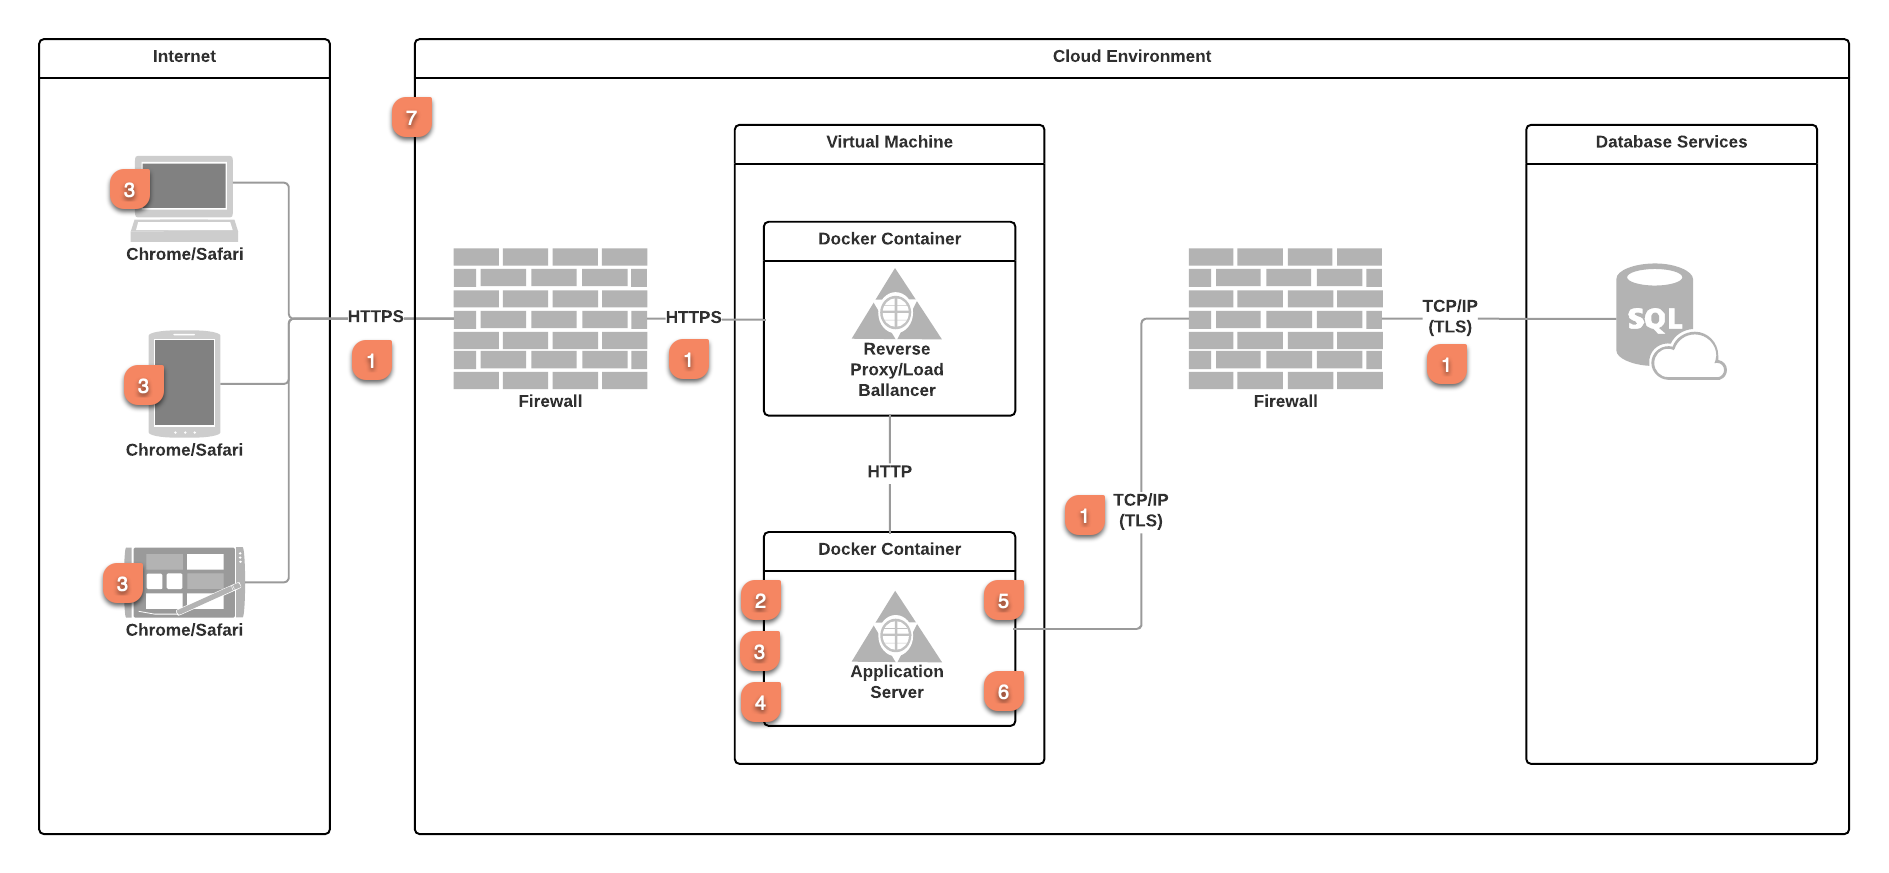
\includegraphics[width=1\linewidth]{images/01-security-diagram.png}
	\caption{A high-level security diagram for TG applications.}\label{sec:01:fig:1}
	\end{figure}

\section*{Secure communication and authentication}\label{sec:02}

\subsection*{Server Authentication for User Protection}

	Application users should be certain that they are accessing the right application on the correct server, and that their communication with the server is secure.
	This basically means three things:

	\begin{itemize}
	\item The server is \emph{authentic}.
	\item The \emph{data integrity} of the communicated information is ensured.
	\item The communication channel is \emph{encrypted}.
	\end{itemize}

	The HTTP protocol over TLS (Transport Layer Security, aka SSL, Secure Sockets Layer) provides a complete solution to the above requirements.
	Thus, HTTPS protocol support by the TG Application Server is the most rigorous solution to the problem of Server Authentication.

\subsubsection*{How HTTPS works}
	Without going into too much detail, it is beneficial to have a general understanding of HTTPS security and how it actually makes communication safe.
	There are two parts to the TLS mechanism.
	One has to do with encrypting the communication channel, the other has to do with certification, which identifies the server as the entity it claims to be. Let's start with channel encryption.

	\paragraph{Channel encryption.}
	The TLS framework employs the use of Asymmetric~\cite{PKC} and Symmetric~\cite{SKC} Cryptography.
	Asymmetric cryptography uses two keys -- public and private -- for encryption and decryption of messages.
	If a message gets encrypted with a private key it can only be decrypted with the corresponding public key, and vice versa.
	The public key, as the name suggests, gets sent to the client application (e.g. a web browser) via an open channel.
	Any eavesdropping adversary would be able to see it, and that is completely fine. The private key remains private to the server.
	So, unless the server is hacked, only the server should be in possession of the private key.

	Thus, once the client has received a public key, all the information encrypted by the client and sent back to the server can only be decrypted by the server.
	However, any information encrypted and sent by the server can be decrypted not only by the client, but also by the eavesdropping adversary, who might have captured the public key during its initial transmission to the client.

	This is where symmetric cryptography comes into place.
	Symmetric cryptography uses a single key for encoding/decoding, and is much faster than asymmetric cryptography.
	Therefore upon receiving a public key, the client generates a key for symmetric cryptography, encodes it with its public key and sends back to the server.
	Thus the key provided for symmetric cryptography would only be decrypted at the server end.
	At this stage both client and server have a shared key and start using it to encode/decode all further communication.
	An eavesdropping adversary would not be able to understand any of the information being communicated in this way.

	\paragraph{Server Certification.}
	Another part of the TLS framework has to do with server identification, and this is where certification plays its role.
	As part of the HTTPS handshake between the client and server, the server presents a certificate of authenticity.
	This certificate has to be signed by a Certificate Authority (CA), or it could be self-signed.

	A client, such as a web browser, has the means for checking whether it can trust the presented certificate.
	If the certificate is signed by a CA, the client checks against its reference of trusted CAs and makes a decision to trust, or not to trust, the presented certificate.
	If the certificate is self-signed, all web browsers would reject it unless it was added to a list of exceptions (i.e. the user explicitly informed the browser to trust the certificate).

	If the certificate is rejected then all communication with the server is stopped, as it could be an imposter trying to emulate the actual server that the client intends to connect to.
	However if the certificate is accepted, the client carries on with an HTTPS handshake (exchanges the keys etc.).

	An interesting thing about CAs is that any organisation (or person for that matter) could become a CA and start signing, for example, its own server certificates.
	Customers may choose to trust a particular not well known CA (e.g. FMS) by adding the corresponding CA certificate to their OS or browser.
	So this all boils down to trust, and has nothing to do with the actual encryption of the communication channel.

	Please note that each server certificate is issued for a single fully qualified domain name (FQDN).
	This information is used by browsers to check that the FQDN part of the URI they are accessing matches the \texttt{Common Name} property of the presented certificate.
	Certificates for different servers should always be issued by signing Public/Private Keys that are unique to those servers (i.e. no server certificate should reuse the same key pair).

\subsubsection*{Communication over HTTPS}

	\paragraph{Java KeyStore.}
	Jetty, which is a Servlet Engine and an HTTP Server used as the basis for TG Application Server, together with Restlet (a framework used for implementing the Resource Oriented architecture of TG Application Server), support TLS infrastructure, and can be configured to enable communication over HTTPS.

	A Java KeyStore (JKS) infrastructure is used for that (as in the case of any Java application) to establish a TLS infrastructure.
	The server's Public/Private Keys and its Certificate, which are used to establish HTTPS communication, are stored in a keystore file.
	A keystore file should be protected by a password. Access to Private Keys, which are stored there, is protected by yet another password.

	The keystore file password is mainly used to check file integrity when accessing it in order to make sure that it was not tampered with.
	It also provides an additional layer of protection in case the keystore file gets leaked or stolen.
	The Private Key password is there to protect the Private Keys that are stored in a keystore file.
	This introduces yet another security layer to protect the most essential information, which is used for establishing secure communication between the client and server software.
	It a keystore gets stolen and cracked then eavesdropping adversaries in possession of this information could easily read all communication, and could even set up a fake server to obtain user names and passwords by redirecting users to the counterfeit service.

	In most cases, the keystore file is located on the same physical server as the application server, and is protected by the underlying OS.
	Thus, if the server security is sound there would be no way to steal the keystore file.

	Another important concern is how to handle passwords to a keystore file and Private Keys.
	One common anti-pattern is to store those passwords in a class file as part of the source.
	This leads to two possible ways for an adversary to access the passwords.
	Firstly, the application source might get stolen (e.g. a GitHub repo gets hacked).
	In this case an adversary would obtain the passwords from the source files.
	Secondly, packed jar files of the application server might get leaked as a result of some (even accidental) security breach (e.g. jar files were uploaded to an insecure FTP server).
	By decompiling classes from jars, an adversary could obtain the passwords.

	The most reasonable option is to provide those password as an application server parameter during its start up.
	Securing application configurations falls into the domain of configuration management, and is usually specific to a deployment environment.

	In addition, different TLS certificates are used for development and deployment purposes, and kept in different keystore files.
	In fact, the deployment keystore file should only be kept at the deployment server, and it would be best if the only person who knows the password to that keystore and Public Keys is the administrator of the deployment server.
	This way the chance of any accidental information leaks would be significantly reduced.

	\paragraph{Let's Encrypt.}
	An alternative to maintaining JKS files is to use Let's Encrypt -- a non-profit certificate authority that provides X.509 certificates for TLS at no charge~\cite{LEC}.
	This approach is arguable more secure and easier to maintain due to an automated process for certificate renewal.
	Also, using this approach fosters better modularity by moving responsibility for maintaining the TLS infrastructure away from the application.
	For example, a reverse proxy such as HAProxy can be responsible for maintaining the TLS infrastructure.
	This approach proved to be reliable in real life production deployments of TG applications, and is recommended as a default option.


\subsection*{Client Authentication for Server Protection}

	The previous section describes a way to protect the user from connecting to an untrusted server and from an eavesdropping adversary listening to the data being exchanged.
	This, however, does not protect the server from being accessed by an interrogative adversary who would want to access the data that is stored at the server side.
	There are no bulletproof methods against user imposters, but there are approaches that would most certainly make it really challenging to break.

	If a server needs to be protected from anonymous access, a client authentication mechanism would need to be put in place.
	Unfortunately, unlike the case of HTTPS, there are no standard reliable HTTP mechanisms for user authentication.
	However, there are very reasonable approaches on top of HTTP that proved to be highly reliable.
	Article ``Dos and Don’ts of Client Authentication on the Web''~\cite{MIT} by MIT Laboratory for Computer Science provides a really good insight into the problem with client authentication and offers one possible solution that was well analysed from different penetration perspectives.
	TG employs a system based on the proposed approach, but with its own modification to further harden the scheme.

	The rest of this discussion is presented in several subsections, each addressing specific concerns of the methodology that was developed for client authentication.

\subsubsection*{Login and 2-factor authentication}
	It is assumed that before the first time any user attempts to login to the system, they've been registered by a system administrator and have been provided with their username.
	No passwords are specified for such first time users.
	After successful registration, each user receives an email advising their registration details and asking them to setup their password.
	\hyperref[sec:02:fig:2]{Fig.~\ref*{sec:02:fig:2}} depicts an example of such an email.

	\begin{figure}[h!tbp]
	\centering
	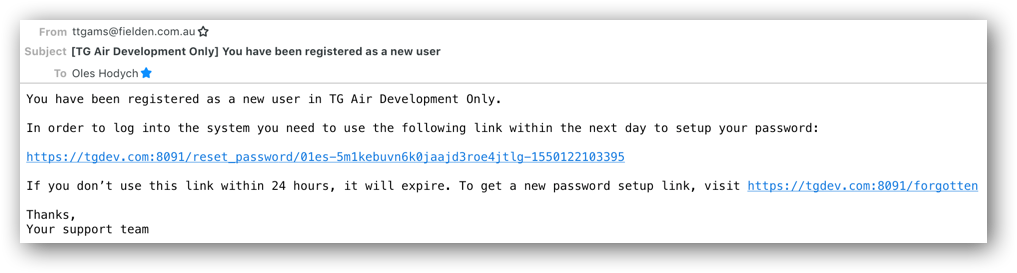
\includegraphics[width=1\linewidth]{images/02-new-user-registration-email.png}
	\caption{An email for a newly registered user.}\label{sec:02:fig:2}
	\end{figure}

	When users access the system, they are presented with a login prompt where they can sign in by entering their credentials or, as it would be in case of first time users, choose to sign up.
	The sign up functionality provides users with a prompt to enter their username (provided to them by a system administrator) and the password of their choosing (see more regarding this in the next subsection).

	In order to validate that the person who is signing up is in fact a valid user and not an imposter, a cryptographically random token gets sent to the user's email address and should be presented by the user to complete the sign up process.
	As the result of successful sign up, the user's system record gets updated with a HMAC-SHA1 hash code of their password.

	Once a user is signed up, they are required to login explicitly.
	Each explicit login can be done in conjunction with 2-factor authentication~(2FA), where the user should enter a one-time passcode generated using HOTP~\cite{HOTP} or TOTP~\cite{TOTP} algorithms.
	The delivery mechanism for passcodes could be an SMS or a mobile app such as Google Authenticator.
	Alternatively, if neither SMS capability nor mobile authentication app is available, there could always be a weaker 1.5-factor authentication put in place, whereby passcodes are provided to users via email.

	Upon login, the user may choose to mark the device that is used for accessing the application as trusted.
	This tells the system not to require explicit login on this device in the future.
	More about this capability is discussed in later sections.

	\paragraph*{Password strength}
	The resilience of user passwords to guessing is one of the essential security aspects.
	If user passwords can be easily guessed then no matter how clever and bulletproof is the rest of the application security subsystem, an adversary would have one less barrier to break before gaining access to the application.
	This would be almost like having no user passwords at all.
	The 2-factor authentication makes this a bit harder for an adversary to use the password without access to the user's phone, but through social engineering this kind of information can also be obtained.
	Therefore, it is best for all parts of the security puzzle if the password is really hard to break or guess.

	There are information entropy based approaches to measuring the strength of passwords (e.g.~\cite{NIST}, \cite{DROPBOX}).
	This approach is both stronger and easier for users to follow when compared with rule-based approaches.
	The lower threshold for password strength in TG applications is configurable.

	The strength of user passwords is only checked when users sign up or change their passwords.
	Password strength is checked at both the client and server sides.
	At the client side users are provided with instantaneous strength estimation feedback upon entering their password.
	\hyperref[sec:02:fig:1]{Fig.~\ref*{sec:02:fig:1}} illustrates the situation where a password entered by a user was recognised as ``strong''.
	This way users know that their passwords are reliable and would not be rejected by the server upon submit.

	\begin{figure}[h!tbp]
	\centering
	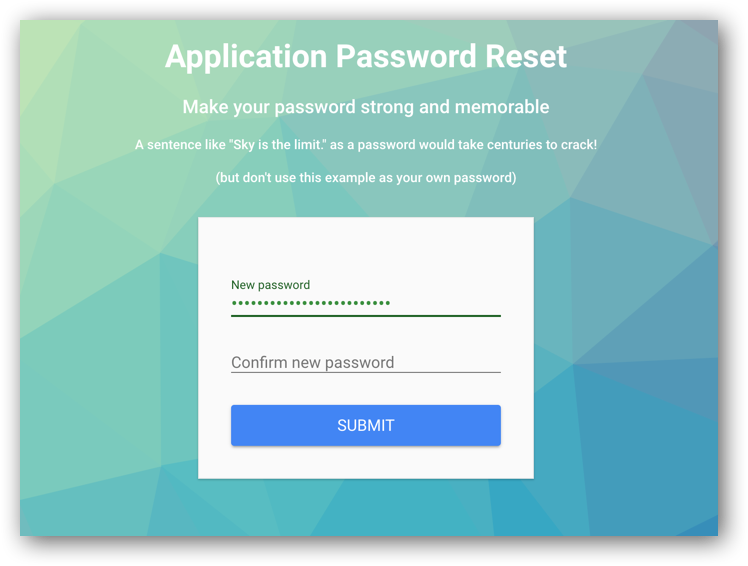
\includegraphics[width=0.6\linewidth]{images/03-new-user-setting-up-password.png}
	\caption{Password strength indication.}\label{sec:02:fig:1}
	\end{figure}

\paragraph*{Preventing rapid-fire login attempts and account lockout.}

	Success of brute force methods for guessing passwords is largely based on the number of passwords that can be fed into the system in a given timeframe.
	If the target application does not restrict the number of passwords that can be presented for a given user, then the password will be guessed very quickly on modern hardware.

	The 2-factor or even 1.5-factor authentication helps a great deal to increase the number of combinations that would need to be presented to the system during a brute force attack.
	However, depending on the computational power used for attacking, such approach could still be practical.

	A better approach would be to slowdown the rate at, which passwords can be presented to the system for a given user.
	For example, three unsuccessful sequential entries for the same user could result in a 1 minute delay before another password could be presented for the same user.
	The delay time may increase exponentially with an increase in the number of unsuccessful sequential tries for the same username.
	Such an approach makes brute force attacks impractical.

	TG applications implement the following rules:
	\begin{itemize}
	\item[--] 3 attempts within the first 15 seconds are permitted without any delay; and
	\item[--] 1 attempt per 15 seconds is permitted after that; and
	\item[--] lockout a user account after 6 unsuccessful attempts.
	\end{itemize}

	In addition, the possibility for timing-based attacks during login to identify valid and invalid users is reduced by performing equivalent computations to take the same time for all login attempts.

\subsubsection*{Restoring or resetting a password}
	The process of password restoring is almost identical to the sign up procedure.
	\hyperref[sec:02:fig:3]{Fig.~\ref*{sec:02:fig:3}} illustrates how users can initiate the password restoring/resetting process by going to ``Forgotten password''~(4), and specifying their user name or email address.

	\begin{figure}[h!tbp]
	\centering
	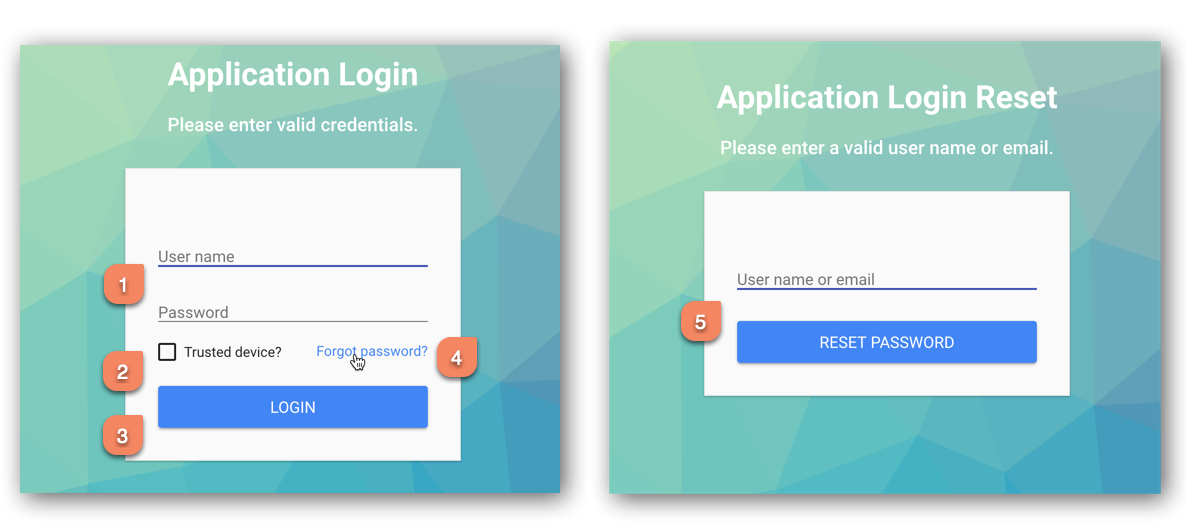
\includegraphics[width=1\linewidth]{images/04-login-or-forgotten-password.png}
	\caption{Restoring a forgotten password.}\label{sec:02:fig:3}
	\end{figure}


	The web page that is presented after submitting a reset request is identical for successful and unsuccessful requests.
	This is required to harden applications against enumerating of valid users or their email addresses.
	\hyperref[sec:02:fig:4]{Fig.~\ref*{sec:02:fig:4}} provides an example of such a web page.
	Further to that, TG applications implement the randomisation of the request/response time that is based on the real-time statistics for valid requests in order to reduce the risk of timing-based attacks whereby response times for valid and invalid users get analysed.

	\begin{figure}[h!tbp]
	\centering
	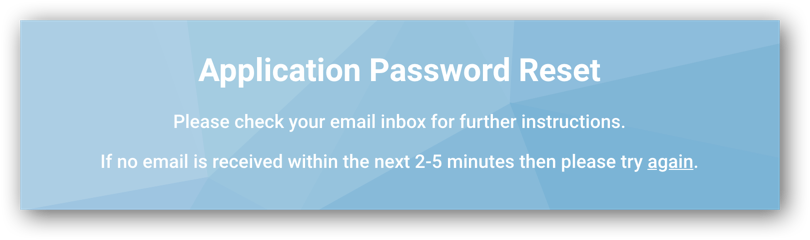
\includegraphics[width=0.7\linewidth]{images/05-password-reset.png}
	\caption{Password reset.}\label{sec:02:fig:4}
	\end{figure}

	If a request to reset their password was submitted successfully, the user should receive an email containing a URI with a cryptographically random token.
	The hash code of this token (but not the token itself) is persisted at the server side against the user, to be used in the password resetting process for validation, and has an expiration time (15 minutes by default).
	Clicking the hyperlink with a valid token loads a web page as in \hyperref[sec:02:fig:3]{Fig.~\ref*{sec:02:fig:3}}, where a new password can be specified.

	As with the sign up procedure, the user needs to log in explicitly after successfully resetting their password.
	At his stage, and if enabled, a 2FA mechanism should require the user to enter a valid passcode.

\subsection*{Reduced Sign-On instead of Single Sign-On}
	A quote from a Wikipedia entry states the following about the very nature of single sign-on~(SSO):

	\begin{quote}
	Single sign-on (SSO) is a property of access control of multiple related, but independent software systems.
	With this property a user logs in once and gains access to all systems without being prompted to log in again at each of them.
	\end{quote}

	SSO implies a mutual trust between multiple software systems that are potentially developed by different vendors.
	If one of such trusted systems gets hacked, the adversary automatically gains access to all other systems in the same SSO circle of trust.

	A widely adopted alternative to this quite vulnerable approach is Reduced Sign-On~(RSO).
	The main idea behind it is to reduce the number of times users need to enter their name and password, but require the users to login explicitly (at least once) to the independent software systems separately.
	This approach is especially applicable for Web-facing software systems, where weakness in one trusted application would give an adversary unrestricted access to the rest of the applications on the same server.

	Although TG applications can be integrated with identity providers (e.g. a corporate ADFS~\cite{ADFS}) by means of SAML~\cite{SAML} to achieve SSO, the default security subsystem in TG applications follows the RSO principle, and employs the concept of \emph{trusted devices} to identify devices where login sessions may remain valid for a long time without the need to explicitly re-authenticate.
	Upon login, users indicate whether their current device (PC, tablet etc.) can be trusted for future sessions.
	If so, session authenticators (discussed below) for those devices would be remembered as \emph{trusted} by the application, and all future attempts to access the application from trusted devices would not require the user to login explicitly again.

	\emph{Untrusted devices} would also not require an explicit login for the duration of an uninterrupted/continuous user session.
	Once the user was logged in, each request to a TG application is recognised as a part of an \emph{uninterrupted} session if the time between sequential requests is sufficiently short (e.g. 5 minutes).
	If a session from an untrusted device expires (e.g. the 5 minute timeframe has lapsed between sequential requests), the user is required to login explicitly again.
	The same is true for trusted devices, but the expiration time is much longer (e.g. days rather than minutes, configurable).

	This approach with trusted and untrusted devices provides a way to accomplish reduced sign-on in different scenarios.
	For trusted devices, it provides users with a convenience almost identical to SSO, whereby users do not need to login repeatedly.
	And at the same time, it provides a convenient and secure way for users to access the application from devices that cannot be fully trusted at times where there is no other alternative (e.g. a computer that is shared between multiple users).

\subsubsection*{Session management}
	Upon a successful user login, the server issues a specially designed token to the client.
	This token is used to automatically authenticate the same user for subsequent requests.
	Such tokens are often referred to as \emph{security tokens} or simply \emph{authenticators}.
	Their main purpose is to protect user passwords by removing the need to transmit the passwords over a communication channel as part of each request.
	This significantly reduces the chances for user passwords to be stolen.
	Authenticators play a key role to designate and track user sessions within the application, and provide a way to differentiate between trusted and untrusted devices.

	\paragraph{Authenticator structure and lifecycle.}
	Authenticators in TG applications consist of a username, series identifier and expiration time, and a hash code of these three parts (HMAC-SHA1), all separated by double colons:
	\begin{verbatim}
	username::series identifier :: expiration time :: HMAC-SHA1
	\end{verbatim}

	The \texttt{username} part should correspond to the name provided by the user upon an explicit login.
	It is considered to be ``easily guessable''.
	That is, any usernames for registered users in the system can be easily obtained by an adversary by means of algorithmic generation.

	The \texttt{series identifier} part is a cryptographically strong random string, which uniquely identifies a user session in a way that is extremely difficult to guess.
	It is used in addition to the username in order to make authenticators more difficult to forge, in a way that is explained a bit later.
	New series identifiers are generated for each request, replacing the previous identifier associated with the corresponding user identifier.
	Series identifiers are persisted into the session table.
	However, to prevent leaking of identifiers in the event of a stolen database, instead of the actual series identifiers, their HMAC codes are stored (the same protection as with user passwords).
	The same username can be associated with several series identifiers in case of several devices being used by the user (e.g. the user's tablet and a workstation).

	The \texttt{expiration time} part holds the unix timestamp (number of milliseconds since 1970-01-01) when the session becomes stale (i.e. expires).
	It allows for a quick check to be performed in order to identify requests against expired sessions without doing any database lookups.
	This is especially convenient due to the RESTful nature of TG applications, which do not keep user sessions at the server side.

	The \texttt{HMAC-SHA1} part is the hash code of the string that is built as a concatenation of the first three parts.
	It is the corner stone of the authenticator's verification to ensure that the presented authenticator is indeed the same as was generated by the system, and was not tampered with.
	Hash codes for authenticators are generated using a secret key (2048 or 4096 bits long), which is known only at the server side.
	Therefore, if at least one character in the authenticator was tampered with, it would be identified immediately.

	As can be deduced from the above, authenticators have several mutually checked layers of protection:
	\begin{itemize}
	\item Series identifiers are cryptographically random and thus difficult to guess in order to forge valid authenticators.
	Even if authenticators get intercepted by an adversary, and are used to synthesise authenticators for other users, then due to series identifier uniqueness this would be automatically recognised as an attack.
	Because series identifier are associated with usernames, it is possible to identify whose authenticators were intercepted or leaked, and a symmetrical protective action could be taken (e.g. invalidate all sessions or even disable user accounts associated with the stolen authenticators until the situation has been investigated).

	\item The use of information hashing as part of authenticators provides a quick and reliable way to verify authenticity of authenticators without any database lookups.
	So even if series identifier/username associations are somehow obtained and new authenticators are forged, the knowledge of a secret key would be required to generate a valid hash code.
	In order to obtain a secret key a sophisticated server attack would be required.
	At the same time, if a secret key gets obtained by an adversary, users would still remain relatively safe due to the use of random difficult-to-guess series identifiers that are required to forge valid authenticators.
	\end{itemize}

	Another important aspect of the authenticator lifecycle is the fact that \texttt{series identifiers} get regenerated upon each request.
	Effectively, by presenting a valid authenticator, a new authenticator gets issued with a newly generated \texttt{series identifier}, and this new authenticator is sent back to the client as part of the response.
	Any previous authenticators for the same user are invalidated.
	This property of authenticators is referred to as \emph{continuity} -- it helps to reduce the risk associated with stolen authenticators.

	\paragraph{Safekeeping of authenticators.}
	Authenticators identify users in exactly the same way as usernames and passwords.
	This means that authenticators need to be protected from being stolen or leaked.

	The most obvious way to steal authenticators would be eavesdropping on the communication channel.
	However, this is avoided by using HTTPS, which should be taken for granted in the case of all TG applications.
	Another, less obvious way, is obtaining authenticators from either the server or the client side, where authenticators have to be persisted for reuse.

	In case of the server side, persisting of authenticators is required for validation.
	This is especially essential to identify stolen authenticators as explained later.
	Safekeeping authenticators at the server side is achieved by hashing their series identifier part before persisting.
	This way, it is impossible to reconstruct the original value by the very nature of cryptographic hashing (hash codes cannot be decoded, they are one way encoding only).
	One needs to have the original value in order to obtain the corresponding hash code.
	Therefore, when a client request presents a series identifier as part of its authenticator, its hash code gets computed and then the hash code is compared against the persisted value.
	It is important to note that such approach also reduces the risk of Remote Timing Attacks~\cite{RTA}.

	For the client request to be authenticated it needs to include a valid authenticator.
	If a client request does not have an authenticator it results in HTTP error 401 (unauthorised).
	This means that once issued by the server, the authenticator has to be persisted also at the client side and be automatically included as part of the request each time the user attempts to access the server.
	This is achieved by means of persistent cookies.

	In order to protect cookies at the client side, mainly from being used in cross-site scripting (XSS)~\cite{XXS} attacks, they are marked as \texttt{HttpOnly} cookies.
	This informs the browser that such cookie should only be accessed by the originating server, and any attempt to access them from client-side scripts is strictly forbidden.
	More about this can be read in~\cite{OWASP_HttpOnly} and in~\cite{HttpOnly}.

	\paragraph{What happens if an authenticator gets stolen?}
	Although, extremely unlikely, it is still possible to envisage a situation where users may have their authenticator stolen.
	In this subsection we'd like to discuss what is the worst case scenario under this condition and what can be done to mitigate such risks.
	There are two possible cases -- an authenticator is stolen from an untrusted devices, and from a trusted device:

	\begin{itemize}
	\item\textbf{Untrusted Device.}
	Due to a very short session life (minutes) for untrusted devices, an adversary can only obtain a still valid session if they have access to the authenticated device immediately after the user performed the last request from that device.
	In this case, an adversary would have full access to the same application functionality and data as the original user.
	Again, this is a very unlikely event, but still possible.

	In order to prevent this from happening, the user must logout from the application once the work they were doing from an untrusted device is completed.
	If this does not happen, it would only be possible to recognise potentially unauthorised access by performing usage pattern analysis (e.g. too intensive system usage due to multiple simultaneous or close to each other requests that are not typical for a normal user activity, the same user may have started using the system from a different device, but there is still some activity associated with another session).

	\item\textbf{Trusted Device.}
	Authenticators on the trusted devices don't expire quickly and therefore represent a higher risk than authenticators on the untrusted devices.
	Due to the use of HTTPS for communication and \texttt{HttpOnly} cookies for storing authenticators at the client side, the only way for an adversary to obtain an authenticator from a trusted device is to have direct access to that device.

	If an adversary, after gaining access, would keep using the same trusted device, then the only way to identify unauthorised access is by analysing the usage patterns as in the case of untrusted devices.
	However, a more likely scenario is where an authenticator is stolen from a trusted device, and then used to access the application from a different device by presenting the stolen authenticator.

	In this case, there are two possible scenarios -- the usage pattern analysis as before, or the legitimate user tries to access the system from the same trusted device from where the authenticator was stolen.
	The latter case can be easily identified as an attack due to the property of continuity for authenticators.
	Basically, if an authenticator verified by HMAC code is presented, but the series identifier is no longer associated with the username due to its regeneration upon every request, then all user sessions would be invalidated and an explicit login required.
	This would prevent the adversary from any further access to the application.
	\end{itemize}

\subsection*{Securing communication between applications and databases}
	The need to secure the connection between web clients and the application server is obvious.
	However, it might be equally important to secure communication between the application server and the database server.
	This is especially relevant for cloud environments where these servers are usually virtual servers and should strictly limit who can and cannot connect to them.

	Most popular RDBMS vendors these days provide capabilities to encrypt client/server\footnote{\emph{Client} is in this case the application server, and \emph{server} is the database server.} communications for increased security.
	For example, Microsoft SQL Server and PostgreSQL natively support TLS, which can be used to encrypt the communication as well as to perform identity verification of clients and servers.
	Alternatively, if for some reason the target RDBMS does not support TLS or setting up the TLS infrastructure for individual applications yields too much administrative overhead, it is always possible to use SSH tunnelling to encrypt the network connection between the application and RDBMS servers.

\section*{Authorisation}\label{sec:03}

	Authorisation represents the next layer of security after authentication.
	It governs \emph{access control} by identifying whether authenticated requests have sufficient privileges to access or execute the functionality of the application that is specified in the request.
	This section discusses how \emph{user roles} and \emph{security tokens} are used by TG applications to manage access control.

\subsection*{User roles and security tokens}

	\paragraph{User Roles.}
	Each application user may have 0 or more roles associated with them.
	Active users should really have at least 1 role.
	Editing data and executing actions, including the majority of the standard actions such as ``Delete'', requires an appropriate user role.
	\hyperref[sec:03_01:fig:1]{Fig.~\ref*{sec:03_01:fig:1}} illustrates an attempt to delete selected entities by a user without a role.
	Upon clicking the ``Delete'' action~(1) and confirming the intent, the user is toasted with a permission error~(2), which can be viewed in an information dialog~(3) by clicking the toast.
	Permission errors are thrown either because the user has no active roles or their roles were not granted access to the corresponding \emph{security tokens}, which are discussed a bit further in this section.

	\begin{figure}[h!tbp]
	\centering
	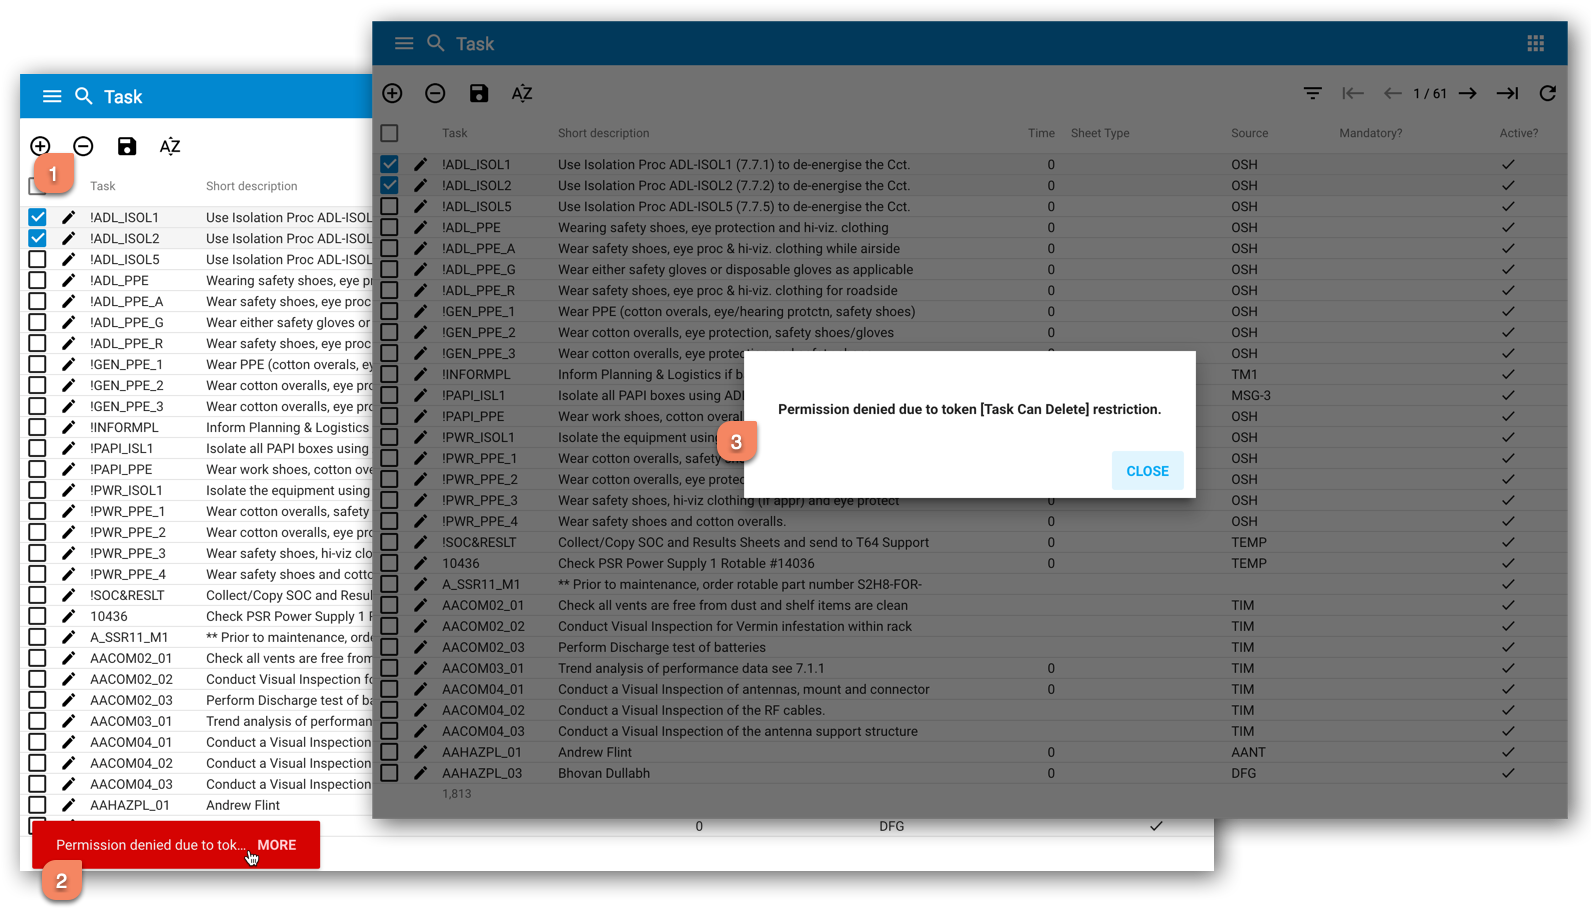
\includegraphics[width=\linewidth]{images/06-permission-denied.png}
	\caption{A permission error for a user with no active roles or the right security token permission.}\label{sec:03_01:fig:1}
	\end{figure}

	\hyperref[sec:03_01:fig:2]{Fig.~\ref*{sec:03_01:fig:2}} shows User Role Centre and Master.
	As can be observed, entity User Role is a very simple activatable entity.
	User roles are defined uniquely by their property ``Role Title'', require a description, and can either be active or inactive.
	It is a good idea to provide a meaningful role description that would convey the role's intent.

	Only active user roles are used as part of the authorisation process.
	Users may have multiple roles and each user needs to have their roles specified separately.
	Inactive roles have no impact on users' permissions (i.e. inactive roles are ignored).
	That is why it may be convenient to simply deactivate a role instead of disassociating that role from each user individually.

	\begin{figure}[h!tbp]
	\centering
	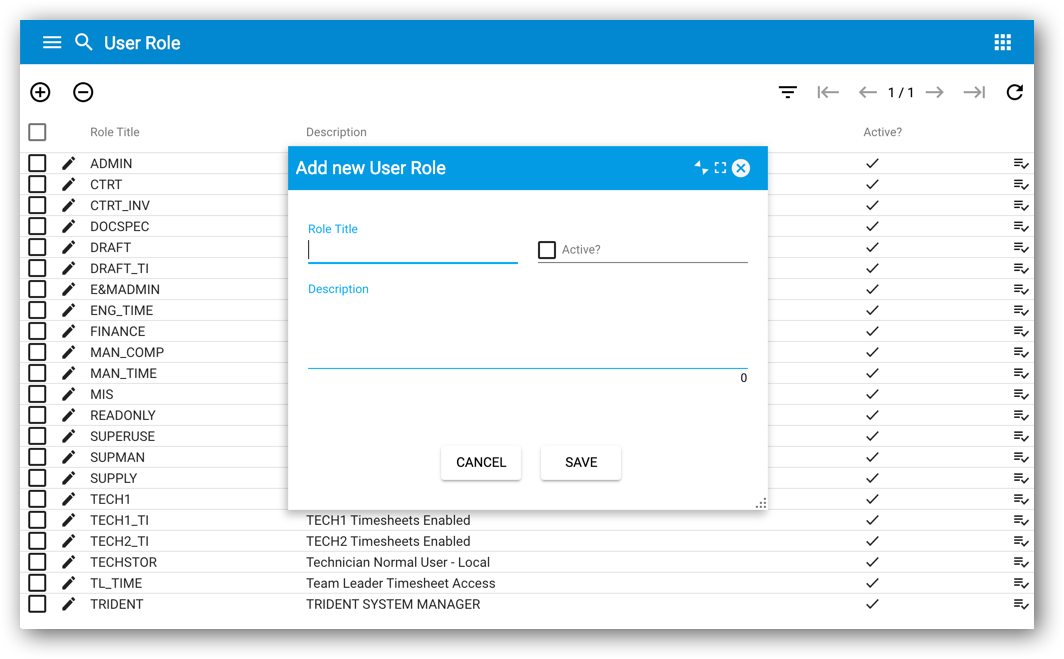
\includegraphics[width=0.8\linewidth]{images/07-new-user-role.png}
	\caption{Adding roles to a user.}\label{sec:03_01:fig:2}
	\end{figure}

	Roles are associated with users by using a secondary action in User Centre.
	\hyperref[sec:03_01:fig:3]{Fig.~\ref*{sec:03_01:fig:3}} depicts ``Add/Remove Roles'' dialog, which appears when the secondary action is clicked~(1).
	Those roles that are already associated with the current user appear at the top of the list as ticked items~(2).
	The rest of the items are sorted alphabetically.
	Roles can be found in the list by either scrolling or searching in the ``Type to search\ldots'' field at the top of the list.
	Searching uses both role titles and their descriptions to find matching values.
	Once the all the necessary roles are ticked, clicking ``SAVE''~(3) saves changes and associates the user with the selected roles.

	\begin{figure}[h!tbp]
	\centering
	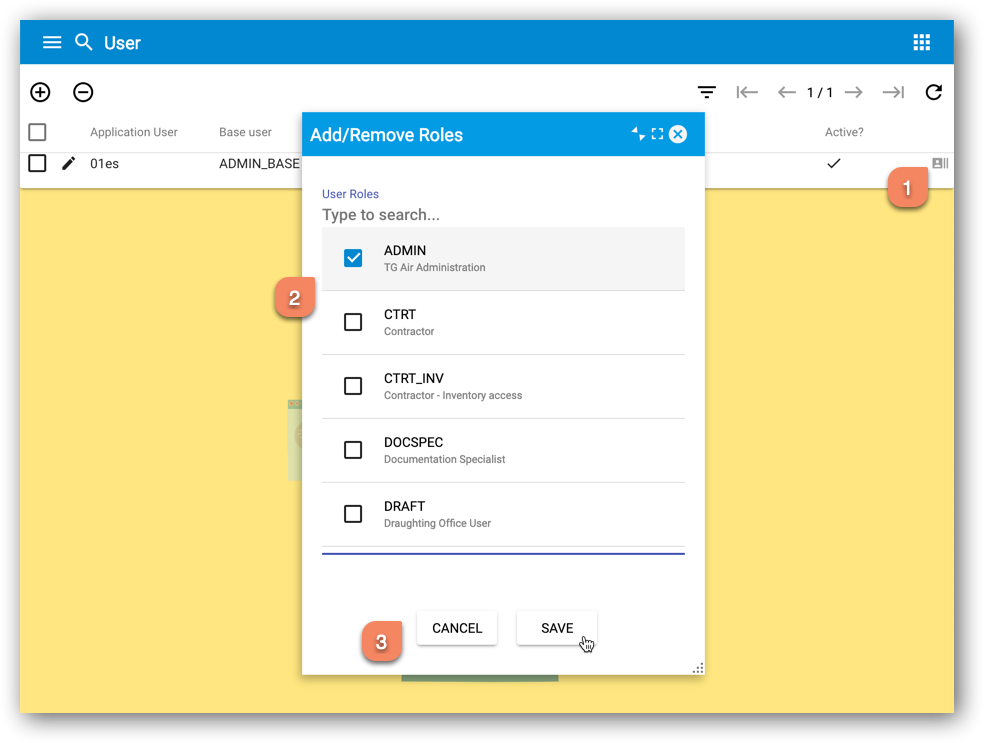
\includegraphics[width=0.8\linewidth]{images/08-adding-roles-to-users.png}
	\caption{Adding roles to a user.}\label{sec:03_01:fig:3}
	\end{figure}

	\paragraph{Security Matrix.}
	\emph{Security tokens} demarcate \emph{authorisation boundaries} within the system, and together with \emph{user roles} they form Security Matrix, which identifies what boundaries are accessible for which roles.
	The union of authorisation boundaries that are accessible to all  \emph{user roles} for a specific \emph{user}, defines authorisation boundaries for that user.

	\hyperref[sec:03_01:fig:4]{Fig.~\ref*{sec:03_01:fig:4}} depicts Security Matrix for a subset of security tokens and roles defined for one of our TG applications.
	Security tokens are represented as a 2-level tree~(1).
	The first level represents logical grouping of security tokens.
	They correspond to application modules.
	Tree nodes on the second level are the actual security tokens.

	\begin{figure}[h!tbp]
	\centering
	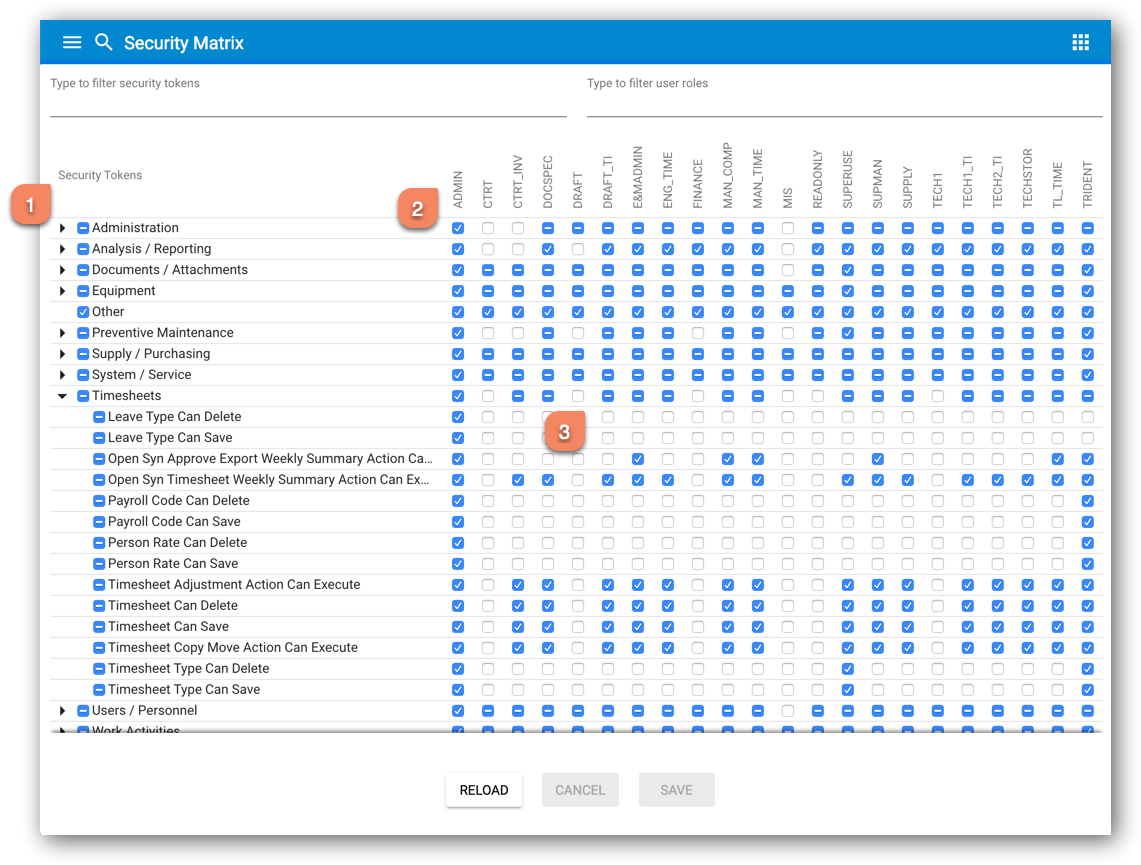
\includegraphics[width=0.9\linewidth]{images/09-security-matrix.png}
	\caption{Security Matrix.}\label{sec:03_01:fig:4}
	\end{figure}

	User roles are represented as columns~(2).
	Both active and inactive roles are displayed.
	The intersection of tree-nodes and columns~(3) is a matrix of actionable checkboxes\footnote{Can be ticked/unticked.}, which identify whether a user role has access to a specific security token or a group of tokens in case an intersection corresponds to a tree node in the first level (i.e. a group).
	Empty checkboxes represent \emph{no access}.
	Ticked checkboxes represent \emph{access}.
	And finally, checkboxes with a ``minus'' icon represent a group access, where some of security tokens are accessible and some are not.

	For example, the checkbox at the intersection of role ``ADMIN'' and module ``Timesheets'' in \hyperref[sec:03_01:fig:4]{Fig.~\ref*{sec:03_01:fig:4}} is ticked.
	As can be easily observed, all security tokens in that group are also ticked for role ``ADMIN''.
	The checkbox at the intersection of role ``CTRT'' and module ``Timesheets'' is unticked -- no security tokens are accessible for this role.
	Role ``CTRT_INV'' has partial access to module ``Timesheets'' -- the checkbox is a ``minus'' and only some security tokens under ``Timesheets'' are ticked.

	The tree with security tokens also has actionable checkboxes to the left of each node.
	Similarly as before, these checkboxes indicate whether a security token, or a group of security tokens, is fully applied (ticked), partially applied (minus) or not applied (empty) to all of the user roles.
	Ticking/unticking these checkboxes affects all visible user roles\footnote{Security Matrix supports filtering by user roles and security tokens. Actioning checkboxes affect only the visible data.}.
	In the case of group nodes, the effect is applied to all visible security tokens in that group and all visible user roles.

	All security tokens belong to 1 of 6 possible authorisation boundary types and each pertains to a separate entity.
	The titles of security tokens identify both an entity and an authorisation boundary that they belong to.
	The following list explains all authorisation boundary types.

	\begin{enumerate}
		\item\textbf{Deletion of Entities} -- an authorisation boundary type that guards deletion of data; titles of security tokens demarcating this type of boundaries contain \texttt{Can Delete}; for example, \texttt{Holiday Can Delete} guards deletion of holidays; some entities such as \texttt{Work Activity} cannot be deleted by their nature, and hence there is no security token \texttt{Work Activity Can Delete}.

		\item\textbf{Saving of Entity changes} -- an authorisation boundary type that guards saving of new and modified data; titles of corresponding security tokens contain \texttt{Can Save}; for example, \texttt{Holiday Can Save} guards saving of new and modification of existing holidays.

		\item\textbf{Modification of Entity properties} -- an type that represents fine-grained authorisation boundaries, guarding changes to individual entity properties; titles of corresponding security tokens contain \texttt{Can Modify}; for example, \texttt{Person Can Modify property [User]} determines if property ``User'' of entity \texttt{Person} can be changed; some user roles may have the authority to change and save changes to any property entity \texttt{Person}, except its property ``User''.

		\item\textbf{Execution of Actions} -- an authorisation boundary type that guards execution of action, be that top-level, primary, secondary or property action; titles of corresponding security tokens contain \texttt{Can Execute}; for example \texttt{Rotable Swap Action Can Execute} guards the ability to execute \texttt{Rotable Swap Action}.

		\item\textbf{Opening Entity Masters} -- an authorisation boundary type that guards the ability to open Entity Masters, be that simple or compound ones; titles of corresponding security tokens contain \texttt{Can Open}; for example, \texttt{Work Activity Master Can Open} guards the ability to open Work Activity Master; users may have the authority to search and view work activities in Work Activity Centre, but may have no authority to load those work activities into the corresponding master; the same security token guards the ability to create new work activities via Work Activity Master.

		\item\textbf{Access to Compound Entity Masters menu} -- an authorisation boundary type that guards access to individual menu items on Compound Entity Masters, effectively providing fine-grained control over what parts of any Compound Entity Master can and cannot be accessed by users; titles of corresponding security tokens contain \texttt{Can Access}; for example, \texttt{Work Activity Master Purchase Orders Menu Item Can Access} guards the ability to access menu item ``Purchase Orders'' on Work Activity Master.
	\end{enumerate}

	Security Matrix provides the ability to filter by security tokens and user roles (case insensitive), which can be convenient when there is a need to work with a specific subset of user roles or security tokens.
	Filtering is performed by matching the values specified anywhere in the security token titles and user role titles.
	Multiple filtering values can be specified by separated them with a comma.

	\hyperref[sec:03_01:fig:5]{Fig.~\ref*{sec:03_01:fig:5}} depicts the result of Security Matrix filtering.
	Field~(1) is used to filter Security Matrix by security tokens, and in this case it contains value ``holiday''.
	Field~(2) is used for filtering by user roles, which is empty.
	As can be observed, Security Matrix displays~(3) only those security tokens that contains value ``holiday'' (highlighted in bold) and the corresponding grouping node.
	All existing user roles (active or not)~(4) are present as there was no filtering applied to them.
	Any changes to security token accessibility would affect only the visible tokens and roles.
	For example, ticking group node ``Administration'' would assign access for all currently visible user roles to all currently visible security tokens.
	Invisible security tokens that belong to the same group would not be affected.

	\begin{figure}[h!tbp]
	\centering
	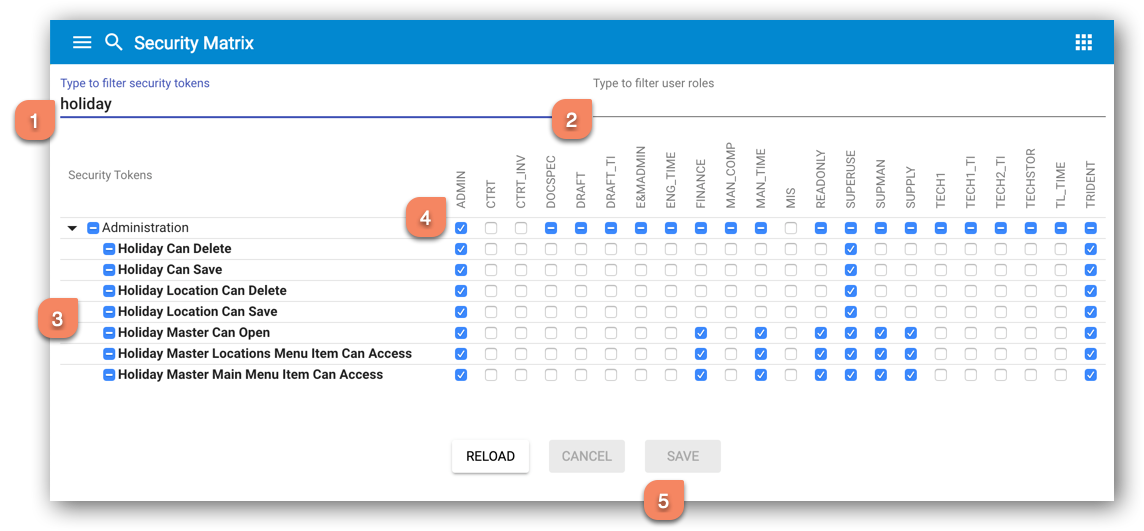
\includegraphics[width=0.9\linewidth]{images/10-security-matrix-filtering.png}
	\caption{Filtering in Security Matrix.}\label{sec:03_01:fig:5}
	\end{figure}

	Changes to security token access rights are recognised by the system immediately after these changes are saved, which can be achieved by clicking button ``SAVE''~(5).
	Security Matrix is a convenient tool where the relationships between multiple security tokens and multiple user roles can be setup and saved in a single transaction.

	As another example of filtering in Security Matrix, \hyperref[sec:03_01:fig:6]{Fig.~\ref*{sec:03_01:fig:6}} depicts the result of filtering by both security tokens and user roles with multiple matching values, which are separated by a comma.

	\begin{figure}[h!tbp]
	\centering
	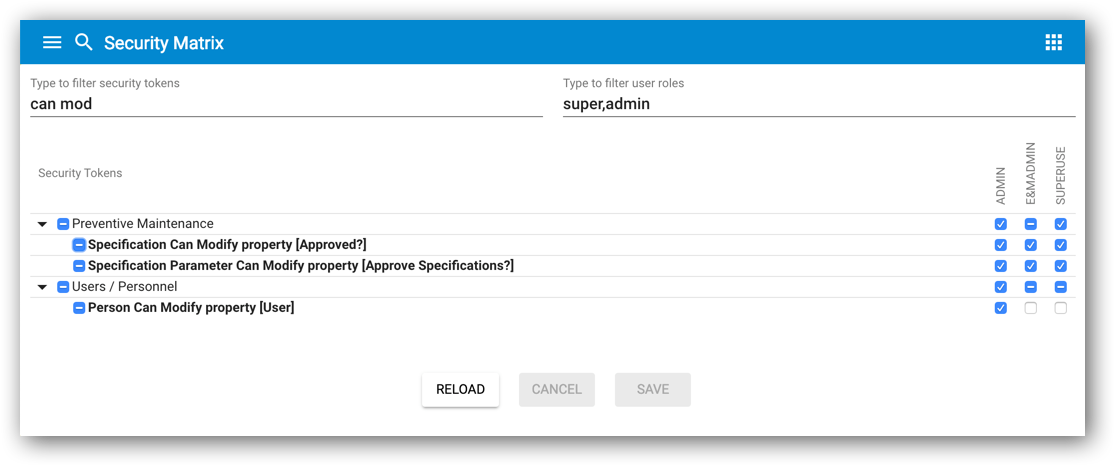
\includegraphics[width=0.9\linewidth]{images/11-security-matrix-filtering-can-modif-and-roles.png}
	\caption{More filtering in Security Matrix.}\label{sec:03_01:fig:6}
	\end{figure}

\section*{Configuration management}\label{sec:04}
	Configuration management is a systems engineering process for establishing and maintaining consistency of a product's performance, functional and physical attributes with its requirements, design and operational information throughout its life~\cite{CM}.
	Until virtualisation was introduced, configuration management of applications and their environments was a complex process with multiple complicated, often manual, steps.
	Ubiquitous use of the cloud as the computing platform of choice led to the development of specialised configuration management tools such as Puppet and Chef.
	Running software in containers such as Docker offers an alternative approach that in many respects is simpler and more reliable.

	We highly recommend using Docker for deploying TG applications.
	This provides a number of benefits:
\begin{enumerate}
	\item Exactly the same image that is tested in the integration development environment is deployed to the User Acceptance Testing (UAT) environment, and then deployed to the production environment.
	\item Deployment consists of simply backing up the database, changing the Docker image tag in the startup script, and then restarting the container/s.
	\item Rollbacks consist of simply restoring the database from the previous backup, changing the Docker image tag to the previous version, and restarting the container/s.
	\item An appropriate Java Runtime and other dependencies are included in the Docker image -- configuration happens at build time rather than deployment time, which significantly reduces system maintenance overheads.
	\item Any TG application can run anywhere that Docker is supported -- all that is needed is a relatively up-to-date Docker installation and a network connection.
	\item Any number of containers can be spun up to cater for increased application load.
	      Unused or idle containers can be spun down to save on infrastructure operating costs.
	\item Distribution of updates is handled by Docker -- no more zipping/unzipping multiple files and copying directories around, or dealing with failed dependency downloads at deployment time.
	\item Initial installation is a breeze -- just a few small changes to a configuration file in a template deployment directory and spin up a new container.
\end{enumerate}

	Deployment environments for Docker vary in functionality and complexity, and can be represented by a single Virtual Machine (VM) with just a couple of Docker containers or a cluster of VMs with hundreds of containers orchestrated by Docker Swarm or Kubernetes.
	Unless an orchestrated Docker environment is readily available, deploying a TG application to a Docker environment with a single VM represents a simple approach that has been proven in a production environment.

	\hyperref[sec:04:fig:1]{Fig.~\ref*{sec:04:fig:1}}~depicts a networking/security diagram for such a simple environment.
	There are two zones on this diagram -- Internet~(1) and Cloud Environment~(2), which could be on-prem or a public cloud.
	Virtual Machine~(3) represents the Docker environment, and Database Services~(4) can be either a database service such as Microsoft Azure SQL, or a database server running, for example, Microsoft SQL Server or PostgreSQL.

	The first Docker container~(5) represents a reverse proxy and a load balancer such as HAProxy.
	In the proposed configuration it is also responsible for TLS termination of web requests (HTTPS)~-- encrypting and decrypting the traffic -- as well as maintaining certificates using the Let's Encrypt service~(8).
	The second Docker container~(6) is the actual TG application.
	Running instances of TG application servers behind HAProxy that is both a load balancer and TLS termination proxy provides an easy way to scale the deployment up when and if required by spinning off new Docker containers.
	This configuration is also well suited for maintaining separate identical environments for UAT, training and production use.

	\begin{figure}[h!tbp]
	\centering
	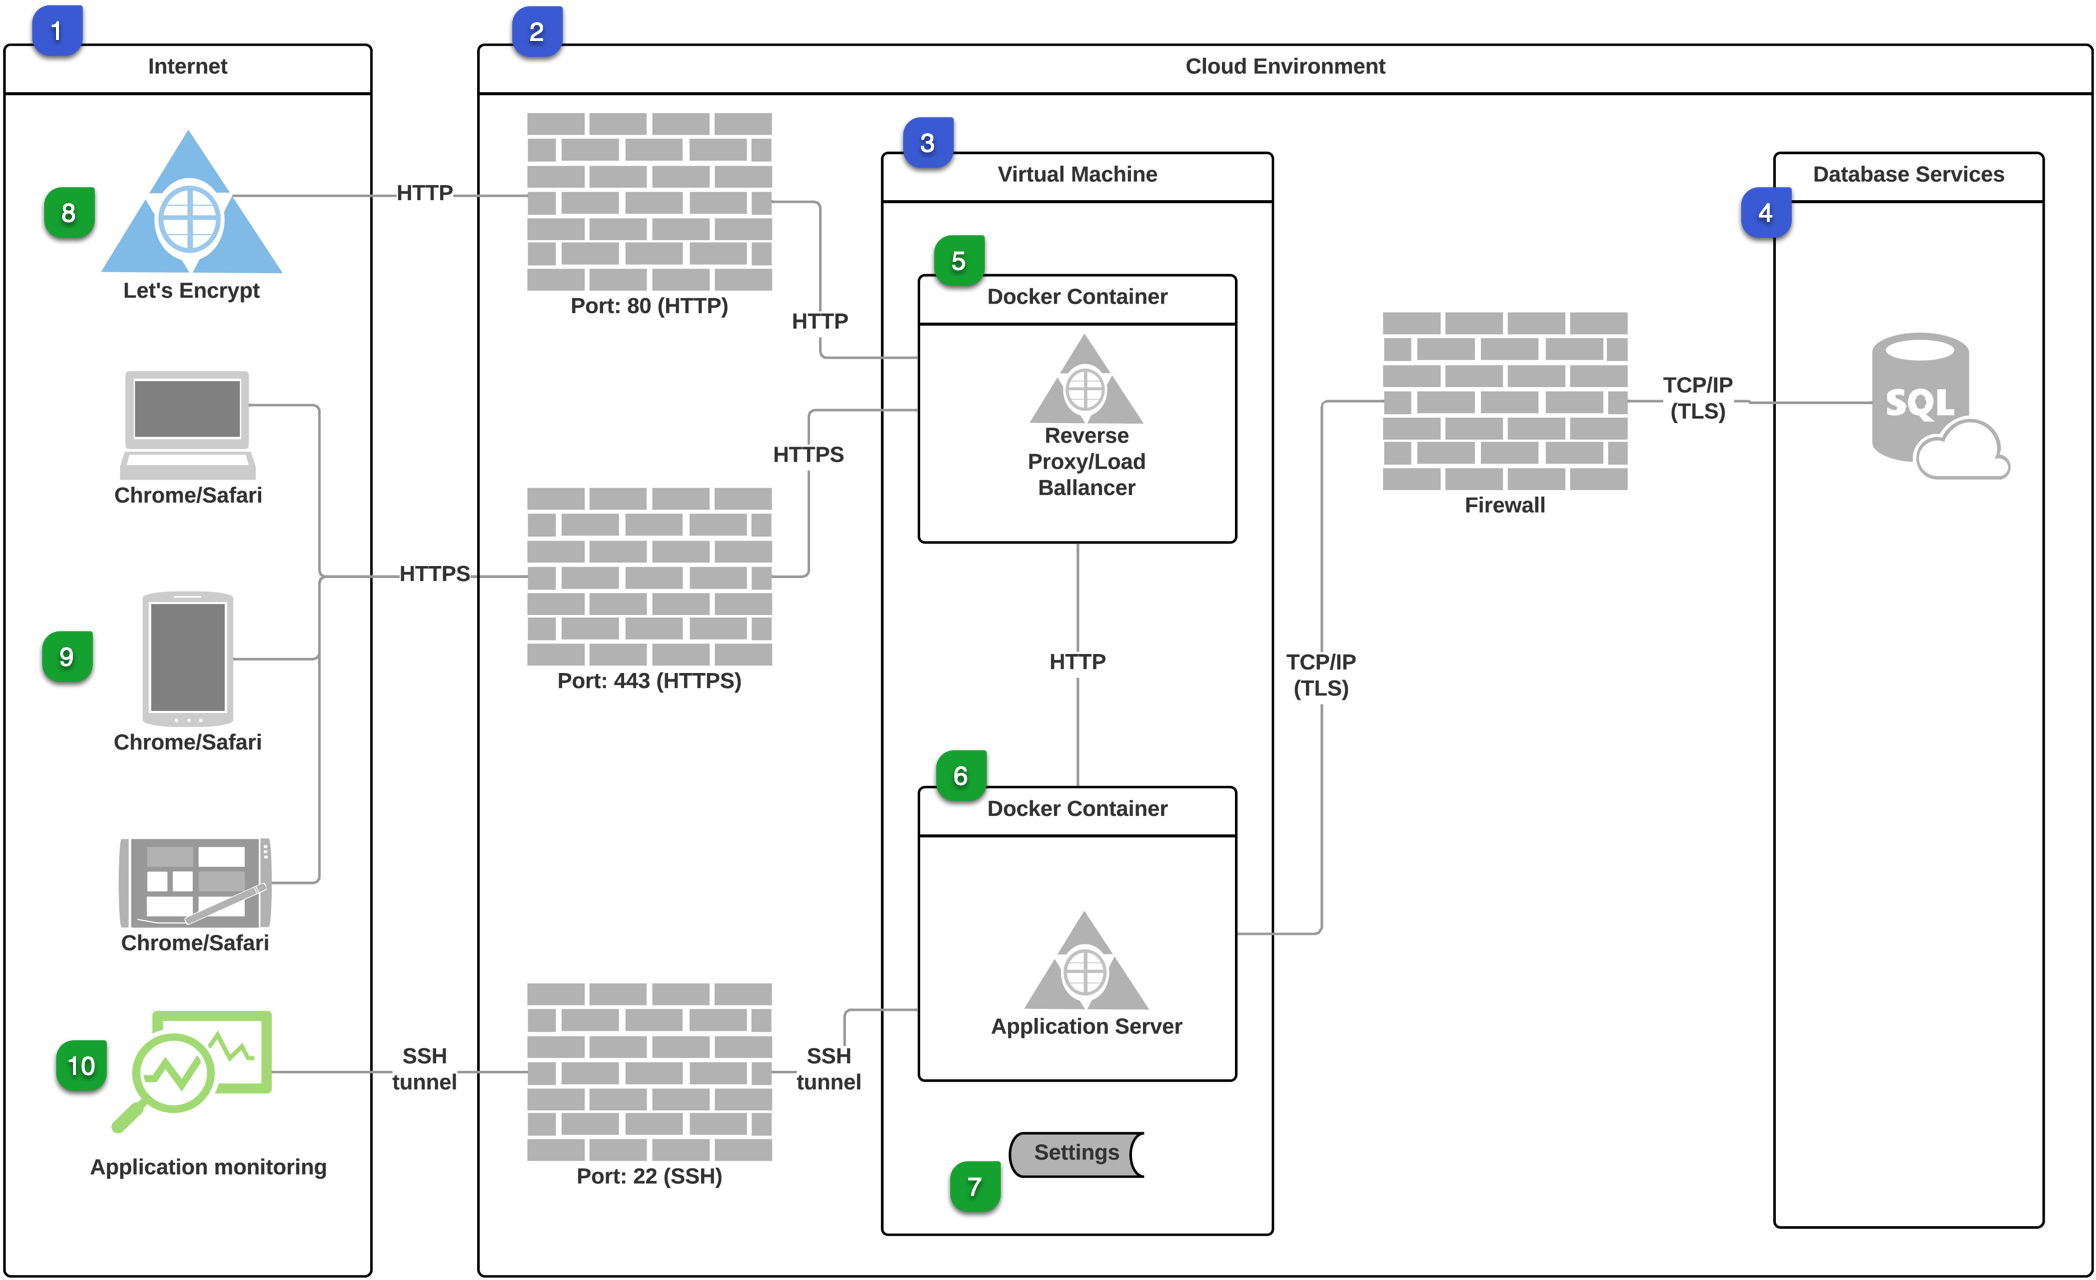
\includegraphics[width=0.99\linewidth]{images/12-more-detailed-security-diagram.png}
	\caption{A single VM Docker deployment environment.}\label{sec:04:fig:1}
	\end{figure}

	Application settings~(7), including DB URI and login credentials, are stored outside the Docker image for a TG application.
	There are several approaches as to how these settings can be passed to the Docker container.
	In the simplest form application settings can be stored in a text file on the VM running Docker containers.
	If the VM can be trusted then this file can potentially be stored as a plain text.
	A better approach would be to encrypt the file in order to avoid accidental unauthorised access to its content.
	A key to decrypt this file would still need to be passed into the TG application.

	More sophisticated approaches for handling application secrets exist and can be utilised if required.
	For example, Docker Swarm secrets~\cite{DSS} or HashiCorp Vault~\cite{HCV}.
	However, these approaches do introduce additional administrative overheads.

	In all cases, communication is tightly controlled by firewalls, which limits both ports and IP addresses that are permitted.
	For example, a secure real-time application monitoring~(10) can be achieved by establishing an SSH tunnel.
	Unlike normal HTTPS traffic(9) that is not limited to specific IP addresses, application monitoring requests should be restricted to a small number of IP addresses.
%
% ---- Bibliography ----
%
\begin{thebibliography}{5}

\bibitem{PKC} Public Key Cryptography,
\href{http://en.wikipedia.org/wiki/Public-key_cryptography}{Online}

\bibitem{SKC} Symmetric Key Cryptography,
\href{http://en.wikipedia.org/wiki/Symmetric-key_algorithm}{Online}

\bibitem{LEC} Let's Encrypt,
\href{https://letsencrypt.org}{Online}

\bibitem{MIT} Dos and Don'ts of Client Authentication on the Web,
\href{https://pdos.csail.mit.edu/papers/webauth:sec10.pdf}{Online}

\bibitem{HOTP} HMAC-based one-time password algorithm,
\href{https://en.wikipedia.org/wiki/HMAC-based_One-time_Password_algorithm}{Online}

\bibitem{TOTP} Time-based one-time password algorithm,
\href{https://en.wikipedia.org/wiki/Time-based_One-time_Password_algorithm}{Online}

\bibitem{NIST} Password strength: NIST special publication 800-63,
\href{http://en.wikipedia.org/wiki/Password_strength#NIST_Special_Publication_800-63}{Online}

\bibitem{DROPBOX} Dropbox approach to passwords,
\href{https://blogs.dropbox.com/tech/2012/04/zxcvbn-realistic-password-strength-estimation}{Online}

\bibitem{SSO} Single Sign-On,
\href{https://en.wikipedia.org/wiki/Single_sign-on}{Online}

\bibitem{ADFS} Active Directory Federation Services,
\href{https://en.wikipedia.org/wiki/Active_Directory_Federation_Services}{Online}

\bibitem{SAML} Security Assertion Markup Language,
\href{https://en.wikipedia.org/wiki/Security_Assertion_Markup_Language}{Online}

\bibitem{RTA} Remote Timing Attack,
\href{http://en.wikipedia.org/wiki/Timing_attack}{Online}

\bibitem{XXS} Cross-site scripting,
\href{http://en.wikipedia.org/wiki/Cross-site_scripting}{Online}

\bibitem{HttpOnly} Protecting your cookies with HttpOnly,
\href{http://blog.codinghorror.com/protecting-your-cookies-httponly/}{Online}

\bibitem{OWASP_HttpOnly} OWASP on HttpOnly,
\href{https://www.owasp.org/index.php/HttpOnly}{Online}

\bibitem{CM} Configuration management,
\href{https://en.wikipedia.org/wiki/Configuration_management}{Online}

\bibitem{DSS} Docker Swarm Secrets,
\href{https://docs.docker.com/engine/swarm/secrets/}{Online}

\bibitem{HCV} HashiCorp Vault,
\href{https://www.vaultproject.io/}{Online}


\end{thebibliography}
%

\end{document}

